	
	\section{Introduction}

	The aim of this thesis is to explore the relatively new field of machine
	learning on graphs. In particular, this thesis will focus on graph machine
	learning applications for the purpose of gaining customer insights. Graph
	machine learning is the current frontier in machine learning and has vast
	applications in many areas as recently shown by the success of AlphaFold
	\citep{senior2020improved}. AlphaFold made a breakthrough for predicting
	protein structures where they made use of the observation that a folded
	protein can be considered as a spatial graph \citep{AlphaFoldTeam2020}. In
	addition, there is a vast range of applications for graphs in the fields of 
	natural science, social science and many more as shown by the excellent 
	overview given by \cite{zhou2020graph}. In principle, graphs are useful 
	whenever one wants to model interactions or relationships.\\

	\subsection{Relevance to Economics}

	\noindent From a business \& economics perspective, graphs are particularly
	interesting if one wants to for instance model the interactions between
	institutions. An example for this is a study published by
	\cite{schweitzer2009economic} which created a graph showing the 
	interdependencies of international banks as a network, see figure 
	\ref{fig:bank_network}. This is a useful representation of interdependencies 
	and is an important basis for making systems more robust. \\

	\begin{figure}[h]
		\centering
		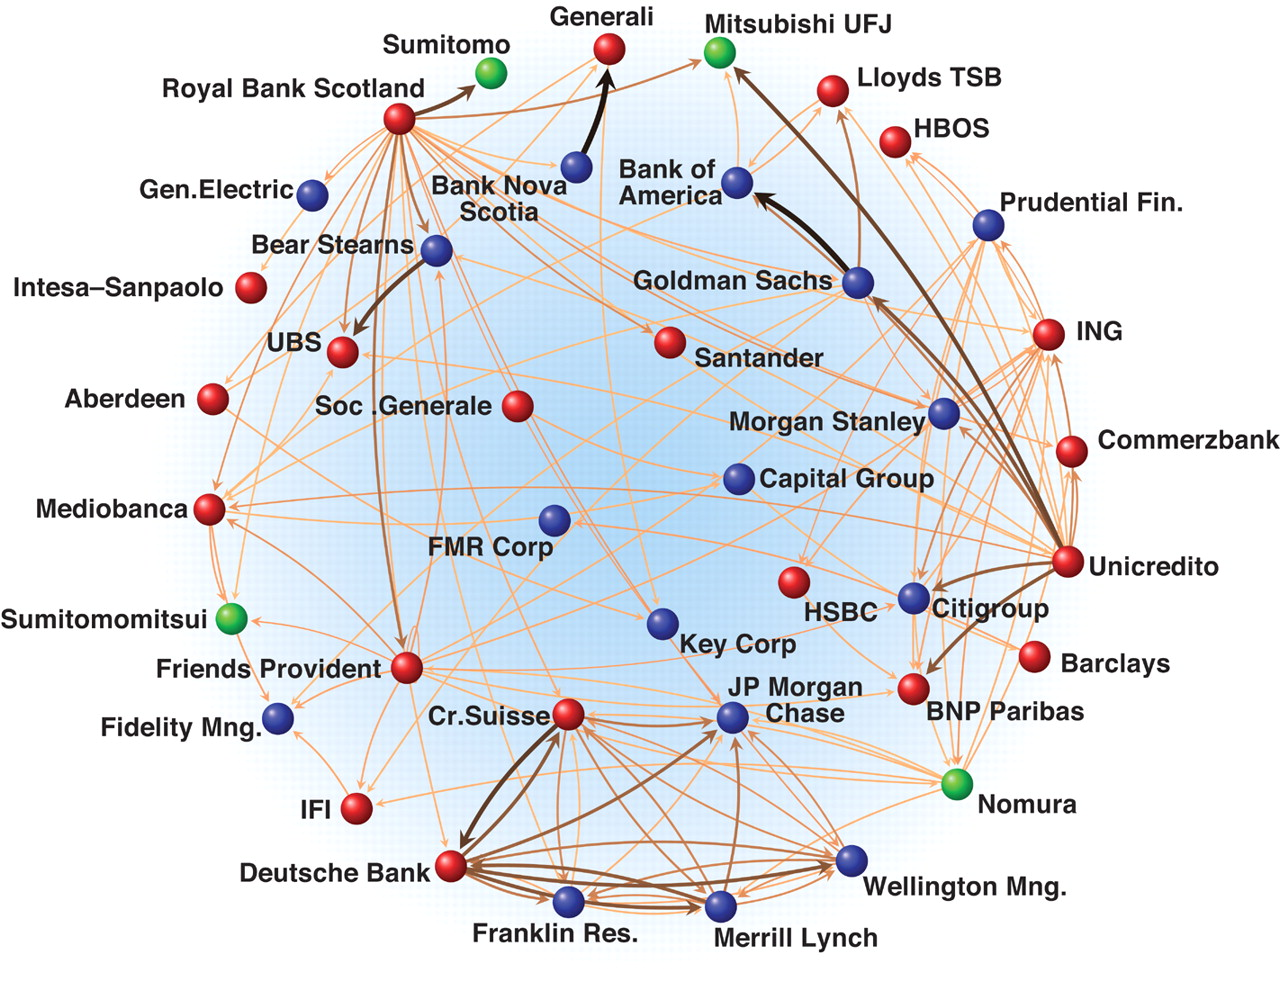
\includegraphics[width=0.5\textwidth]{bank_network.jpg}
		\caption{Bank Network}
		\cite[p. 424]{schweitzer2009economic}
		\label{fig:bank_network}
	\end{figure}

	\noindent Another interesting application of graphs for business \& 
	economics are social interactions. While there are many different types of
	social interactions of interest, social interactions for marketing
	purposes have been among the most popular. Indeed, this is one of the main
	areas where social networks such as Facebook or search providers such as 
	Google make their revenue by selling advertising 
	\citep{Facebook2021,Alphabet2021}. Both Facebook and Google have the advantage, 
	that their businesses naturally capture relational or more generally network 
	data which can be represented as graphs. Most researchers or companies however 
	do not have access to such data. Companies for instance may have access to large
	amounts of customer data, however they typically would not have access to
	relational information (e.g. which client is connected with which other
	clients). The same is true for researchers, where social scientists
	often collect data via anonymous surveys. It is important to
	highlight, that there is a lot of social network data available online. 
	This network data however typically only contains the network structure. 
	The feature data of the people present in the network is however typically not
	provided. This is an issue in terms of data access. \\
	
	\subsection{Research Topic}

	\noindent Given the difficult access to graph data, this thesis will
	explore to what extent synthetic graphs can be generated using real-world
	cross-sectional data. An example for such data could be the client database
	of a company. The aim is then not only to generate graphs but to test 
	whether the resulting graph can be used for meaningful machine learning tasks. 
	In order to test this, appropriate datasets will be selected. It would of 
	course be best, if one would have access to real graph data. If graph data 
	had been available for an appropriate application, this would have been 
	preferred for this thesis. The absence of such available graph data and the 
	difficulty of generating / collecting real graph data sparked the interest 
	and research topic for exploring synthetic graph generation for subsequent 
	machine learning tasks. If this application proves to be successful, this 
	could provide an alternative and hopefully successful approach for analyzing 
	cross-sectional data. In order to assess, whether synthetic graphs based on real
	cross-sectional data is a viable approach, the results of graph machine
	learning methods will be compared to "standard" machine learning methods.
	This leads to the research question formally presented in the following
	section.

	\subsubsection{Research Question}

	The research question for this thesis is defined as follows:

	\begin{quote}
		\item \textbf{To what extent are synthetic graphs based on real cross-sectional
			data useful for machine learning tasks?}
	\end{quote}

	\noindent In terms of machine learning task, this thesis will focus on a
	classification task. This ensures that the results of the graph machine
	learning methods versus the "standard" machine learning tasks can be
	compared.

	\subsection{Literature Review}

	An extensive literature review was conducted. To the best knowledge of the
	author, there are no other published studies which investigate the
	applicability of synthetic graphs based on real cross-sectional data for
	the purpose of machine learning. The literature review revealed the
	following related literature.
	\\

	\noindent A large related research area is regarding synthetic 
	graph generation. Classical models include the famous Erdös-Rényi graph
	generation model \citep{erdos2011evolution}, the small-world model by
	Watts and Strogatz \citeyearpar{watts1998collective} or the model by
	\cite{barabasi1999emergence}. More recent approaches include Kronecker Graphs 
	\citep{leskovec2010kronecker} and its genralization 
	Multiplicative Attribute Graphs (MAG) \citep{kim2012multiplicative}. 
	MAG work well in that it follows commonly observed network properties observed 
	in real networks as outlined in the paper by Kim \& Leskovec
	\citeyearpar{kim2012multiplicative}. 
	For the purpose of this thesis the MAG model will be used for transforming 
	cross-sectional data into a graph. A more detailed introduction of the MAG 
	model will be given in the theory section. Recently, synthetic graph generation 
	models have shifted to deep generative models. Prominent models include 
	GraphRNN by \cite{you2018graphrnn} or the deep generative model presented
	by \cite{li2018learning}. These models differ to the traditional graph
	generation models in that they learn to create synthetic graphs based on
	real graph samples. These newer approaches could for instance be used for
	drug molecule discovery among many other approaches. These newer models are
	however not purposeful for this thesis. 
